In this thesis, partial state is implemented in Noria~\cite{noria}, a stateful,
dynamic, parallel, and distributed dataflow system designed for the storage,
query processing, and caching needs of typical web applications. Because of the
strong connection between Noria and partial state, this chapter describes the
design and implementation of Noria in sufficient depth to follow the remainder
of the thesis.

\section{High-level Overview}

\begin{listing}[h]
  \begin{minted}{sql}
/* base tables */
CREATE TABLE stories
  (id int, author int, title text, url text);
CREATE TABLE votes (user int, story_id int);
CREATE TABLE users (id int, username text);
/* internal view: vote count per story  */
CREATE INTERNAL VIEW VoteCount AS
  SELECT story_id, COUNT(*) AS vcount
    FROM votes GROUP BY story_id;
/* external view: story details */
CREATE VIEW StoriesWithVC AS
  SELECT id, author, title, url, vcount
    FROM stories
    JOIN VoteCount ON VoteCount.story_id = stories.id
   WHERE stories.id = ?;
  \end{minted}
  \caption{Noria program for a key subset of the Lobsters news
           aggregator~\cite{lobsters} that counts users' votes for stories.}
  \label{f:vote-src}
\end{listing}

Noria runs on one or more multicore servers that communicate with clients and
with one another using RPCs. A Noria deployment stores both \emph{base tables}
and \emph{derived views}. Roughly, base tables contain the data typically stored
persistently, and derived views hold data an application might choose to cache
to improve performance. Compared to conventional database use, Noria base tables
might be smaller, as Noria derives data that an application may otherwise
pre-compute and store denormalized in base tables for performance. Views, by
contrast, will likely be larger than a typical cache footprint, because Noria
derives more data, including some intermediate results. Noria stores base tables
persistently on disk, either on one server or sharded across multiple servers,
but stores views in server memory.

Noria's interface resembles parameterized SQL queries. The application supplies
a \emph{Noria program}, which registers base tables and views with parameters
supplied by the application when it retrieves data. Figure~\ref{f:vote-src}
shows an example Noria program for a news aggregator application where users can
vote for stories (\texttt{?} is a parameter). The Noria program includes base
table definitions, \emph{internal} views used as shorthands in other
expressions, and \emph{external} views that the application later queries. It
can be thought of as an extended schema for the application that includes its
queries. Noria supports much, but not all, SQL syntax.

To retrieve data, the application supplies Noria with an external view
identifier (e.g., \texttt{StoriesWithVC}) and one or more sets of parameter
values. Noria then responds with the records in the view that match those
values. To modify records in base tables, the application performs insertions,
updates, and deletions, similar to a SQL database. Data is represented as
structured records in tabular form~\cite{spanner, bigtable}.

Noria differs substantially from traditional databases in how queries are
executed. Rather than compute a query's results on demand when the
application executes it, Noria does so when the query view is defined.
Noria then caches, or \emph{materializes}, the contents of that view, and serves
queries to that view directly from that cache. To keep the materialized current,
Noria internally instantiates a dataflow program to continuously process the
application's writes and update the views as appropriate.

This kind of view materialization makes Noria particularly well-suited for
read-heavy applications that tolerate eventual consistency, since it shifts
query execution cost from reads, which are frequent, to writes, which are
infrequent. Noria focuses entirely on relational operators, rather than the
iterative or graph computations that are the focus of other dataflow
systems~\cite{naiad, differential-dataflow}.

The application may change its Noria program to add new views, to modify or
remove existing views, and to adapt base table schemas. Noria expects such
changes to be common and aims to complete them quickly, without restarting the
dataflow engine.

\section{Dataflow Execution}

To keep its materialized views from growing stale as the underlying data
changes, Noria uses dataflow. Noria compiles all the application queries into a
joint dataflow program, which it routes all application writes through. The
dataflow is a directed acyclic graph of relational operators such as
aggregations, joins, and filters. Base tables are the roots of this graph, and
external views form the leaves. Noria extends the graph with new base tables,
operators, and views as the application adds new queries.

When an application write arrives, Noria applies it to a durable base table and
injects it into the dataflow as an \emph{update}. Operators process the update
and emit derived updates to their children; eventually updates reach and modify
the external views. Updates are \emph{deltas}~\cite{roll, differential-dataflow}
that can add to, modify, and remove from downstream state. For example, a count
operator emits deltas that indicate how the count for a key has changed; a join
may emit an update that installs new rows in downstream state; and a deletion
from a base table generates a ``negative'' update that revokes derived records.
Negative updates remove entries when Noria applies them to state, and retain
their negative ``sign'' when combined with other records (e.g., through joins).
Negative updates hold exactly the same values as the positives they revoke and
thus follow the same dataflow paths.

Noria supports \emph{stateless} and \emph{stateful} operators. Stateless
operators, such as filters and projections, need no context to process updates;
stateful operators, such as count, min/max, and top-$k$, maintain state to avoid
inefficient re-computation of aggregate values from scratch. Stateful operators,
like external views, keep one or more indexes to speed up operation. Noria adds
indexes based on \emph{indexing obligations} imposed by operator semantics; for
example, an operator that aggregates votes by user ID requires a user ID index
to process new votes efficiently. Noria's joins are stateless, but require that
the state of their inputs be materialized to allow an update arriving at one
input to join with all relevant state from the other.

\subsection{Example Execution}

\begin{figure}[t]
  \centering
  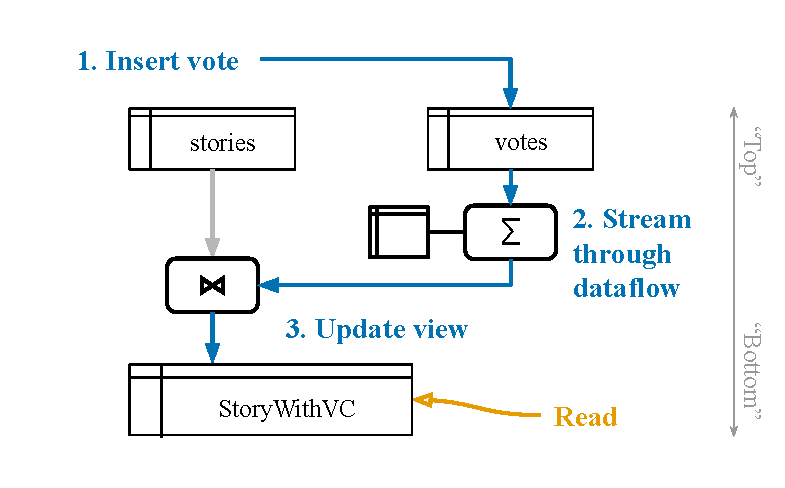
\includegraphics{diagrams/Example Execution.pdf}
  \caption{Noria's dataflow program to maintain Listing~\ref{f:vote-src}. Text
  describes the update path highlighted in blue.}
  \label{f:example-exec}
\end{figure}

Figure~\ref{f:example-exec} shows the dataflow that Noria constructs for
maintaining the Noria program in Listing~\ref{f:vote-src}. At the top are the
entry points into the dataflow\,---\,the operators that represent the schema
base tables\,---\,one for the \texttt{stories} table, and one for the
\texttt{votes} table. Connected to the \texttt{votes} table is a counting
aggregation operator ($\sum$), which corresponds to the internal
\texttt{VoteCount} view. It then feeds into a join operator ($\bowtie$), which
in turn connects to the external \texttt{StoryWithVC} view.

To understand how Noria uses this program to maintain the external view,
consider what happens when a new vote is inserted into \texttt{votes}. The
insertion is introduced into the dataflow as a single-row update with a positive
sign at the \texttt{votes} operator. It stores the update to durable storage,
and then forwards the update as-is to its children; in this case, the count
operator.

The count operator performs a lookup into its own output state for the current
count of the new row's group by column value. The semantics of a count is that
an insertion increments that number by one, so the operator emits a replacement
update for the old state. In particular, the update it produces contains a
negatively-signed record for the old count, and a positively-signed record for
the update count. The replacement also includes the group by column value.

When the join operator receives this replacement update from the count, it
performs a lookup into its other ancestor, \texttt{stories}, for records that
match the join column value of each record of the incoming update. In this case,
both records (the negative and the positive) have the same story identifier as
the join value, so only a single record is returned\,---\,the matching story.
The operator then joins each record in the update with each matching result.
This produces an update that (still) contains one negative and one positive
record, but where each record now includes additional columns from the
\texttt{stories} table.

Ultimately, this two-record update arrives at the operator that represents the
external \texttt{StoryWithVC} view. The changes from the update are applied one
by one, with the negative record removing the entry in the view with the old
vote count, and the positive record adding the replacement entry. Once the
update has been applied, the changes are made visible to readers who will then
start seeing the updated vote count for the story in question.

\section{Consistency Semantics}

To achieve high parallel processing performance, Noria's dataflow avoids
global progress tracking or coordination. An update injected by a base table
takes time to propagate through the dataflow, and the update may appear in
different views at different times. Noria operators and the contents of its
external views are thus \emph{eventually-consistent}. Eventual consistency is
attractive for performance and scalability, and is sufficient for many web
applications~\cite{eventually-consistent, memcached-facebook, pnuts}.

Noria does ensure that if writes quiesce, all external views eventually hold
results that are the same as if the queries had been executed directly against
the base table data. Making this work correctly requires some care. For example,
like most dataflow systems, Noria requires that operators are deterministic
functions over their own state and the inputs from their ancestors. Furthermore,
operators must be distributive so that evaluating the query using
tuple-at-a-time processing is equivalent to evaluating the whole query at once.
Noria operators must also be commutative so that operators with multiple inputs,
like unions and joins, can process their inputs in any order without
coordination.%
\footnote{Maintaining eventual consistency with partial state requires
additional mechanisms, as discussed in \S\ref{s:practical}.}
The standard relational operators that Noria supports all have this property.

\paragraph{Transactions.}
Web applications sometimes rely on database transactions, e.g., to atomically
update pre-computed values. Noria does not implement transactions, though its
support for derived views often obviates the need for them. For example, web
applications often use transactions to keep denormalized schemas synchronized: a
``like count'' column in the table that stores posts or an ``average rating''
column in the table that stores products. Noria obviates the need for such
denormalizations, and the transactions needed to maintain them, by automatically
ensuring that computed derived values are kept up to date with respect to the
base data.

\section{Parallelism}

Servers have many cores, and any high-performance system must be able to take
advantage of multiple cores to take full advantage of the hardware. Noria does
so in several ways. First, it allows reads to happen independently from any
number of threads concurrently. Second, it allows different threads to process
writes in disjoint parts of the dataflow concurrently. And third, it supports
sharding individual operators, or cliques of operators, so that multiple threads
can process disjoint subsets of the data concurrently through the same dataflow
segment. These three mechanisms are described further below.

\subsection{Read Independence}

Since Noria is primarily oriented towards read-heavy workloads, its architecture
is optimized for allowing reads to go ahead at full speed whenever possible. In
particular, Noria does not synchronize reads with reads \emph{or} writes. Unless
a read encounters missing partial state, it never blocks waiting for another
thread.

This is achieved through a concurrency primitive that maintains two instances of
each materialized view, with deduplication between them. Reads go to one view,
and writes to the other. Readers only see updates to the view when a writer
exposes those changes explicitly\,---\,the writer flips an atomic pointer to the
other view, and then waits for all readers to exit the old view before modifying
it again. This can be done on every update, as Noria currently does, or only
occasionally to amortize the cross-core communication penalty. Crucially,
readers do not take locks, and generally operate only on core-local cache lines.

This design allows Noria to use any number of threads to serve reads from any
view. As long as there are cores available, new threads can be added to perform
view lookups and request serialization and deserialization.

\begin{inprogress}
  This design is further discussed in Appendix B?
\end{inprogress}

\subsection{Partitioning}

As part of dataflow planning, Noria divides the dataflow graph into a number of
sub-graphs called \textit{thread domains}. Only a single thread can process
updates in a given thread domain at a time (except with sharding; see below),
and any update that enters a thread domain is processed to completion within
the domain before another update is processed.

State is never shared between thread domains, which means no locks are needed.
Thread domains only ever communicate with one another through messages sent
across the edges of the dataflow, or in the case of upqueries, by sending
messages through dedicated upquery paths set up by the partial subsystem. All
such communication can happen either over the network if the other thread domain
is on a different host, or over an in-memory channel if it is local.

Since thread domains share nothing, some state may be duplicated across
boundaries. For example, a join operator at an incoming edge of a thread domain
must be able to perform lookups into the state of its ancestor, which sits in a
different thread domain. In such a case, Noria will create a thread-local copy
of the join's ancestor's state that it can use locally. Noria's thread domain
assignment heuristics will attempt to draw domain boundaries  such that this
kind of duplication is unnecessary. For example, it will prefer drawing a domain
boundary just before an aggregation (which does not need to look up in the state
of its ancestor), and avoid drawing a domain boundary just before a join.

\subsection{Sharding}

To accommodate applications with such a high volume of writes that the
processing at a single operator is a bottleneck, Noria supports sharding an
operator. Multiple threads split the work of handling updates to a sharded
operator, and operate like independent, disjoint parts of the dataflow.

Noria implements static hash partitioning: how an operator is sharded is
determined when it is added to the dataflow, and does not change over the
runtime of the application. Sharding by value ranges and adjusting the sharding
dynamically is left for future work.

Noria shards operators primarily based on how they access state. For example, an
aggregation performs lookups into its own state, and is sharded by the key
column of those lookups. Any other sharding would mean that processing one
update would require coordination among all shards. A join is sharded by the
join key for the same reason. Base tables are sharded by the table's primary
key. Operators that do not perform lookups (e.g., unions) continue the sharding
of their ancestors to avoid unnecessary shuffles.

To shard an operator, Noria introduces two additional nodes in the dataflow: a
\emph{sharder} placed upstream of the sharded operator, and a \emph{shard
merger} downstream of it. The sharder routes incoming updates to the appropriate
shard of the sharded operator, and the shard merger is a union operator that
combines the output of all the shards to a single downstream output stream.
Noria then eliminates unnecessary sharders and shard mergers, such as if an
operator and its ancestor are sharded the same way.

Sharding boundaries are naturally also thread boundaries, though two connected
thread domains may also be sharded differently. Or, phrased differently, Noria
may partition a chain of operators that are all sharded by the same column into
multiple thread domains to increase parallelism.

\begin{comment}
  Sharding is tracked based on "ultimately source column". (column tracing)
\end{comment}
